\documentclass[11pt, a4paper]{article}
\usepackage[utf8]{inputenc}
\usepackage[T1]{fontenc}
\usepackage{helvet}
\renewcommand{\familydefault}{\sfdefault}
\usepackage[table]{xcolor}
\definecolor{schoolgreen}{HTML}{92D050}
\usepackage{geometry}
\geometry{landscape, margin=2cm, top=4cm, headheight=2.5cm, headsep=0.5cm}
\usepackage{array}
\usepackage{longtable}
\usepackage{graphicx}
\usepackage{fancyhdr}

\pagestyle{fancy}
\fancyhf{}
\fancyhead[L]{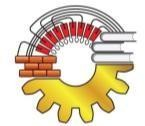
\includegraphics[height=2cm]{../../distritos/4117/templates/logo1.jpg}}
\fancyhead[R]{
\includegraphics[height=2cm]{../../distritos/4117/templates/logo2.jpg}}
\fancyhead[C]{\fontsize{10}{12}\selectfont \textbf{\textit{ESCUELA N.° 4-117 EJÉRCITO DE LOS ANDES \\ DIRECCIÓN DE EDUCACIÓN TÉCNICA Y TRABAJO \\ SECCIÓN V}}}
\renewcommand{\headrulewidth}{0pt}

\begin{document}

\noindent\colorbox{schoolgreen}{\begin{minipage}{\dimexpr\textwidth-2\fboxsep}\centering \textbf{\fontsize{14}{16}\selectfont PROGRAMA 2026}\end{minipage}}

\vspace{1em}

\begin{flushleft}
\textbf{Espacio Curricular:} Termodinámica y Máquinas Térmicas \\
\textbf{Ciclo Lectivo:} 2026 \\
\textbf{Curso:} 5to 2da \\
\textbf{Profesor/a Responsable:} Ferreyra Gustavo David
\end{flushleft}

\vspace{1em}

\begin{longtable}{|p{\dimexpr\textwidth-2\tabcolsep-2\arrayrulewidth}|}
\hline
\rowcolor{gray!20} \textbf{Contenidos Programáticos} \\
\hline
\textbf{EJE Nº 1: FUNDAMENTOS TÉRMICOS Y SISTEMAS} \\
$\bullet$ Transmisión de calor: Conducción, Convección y Radiación. \\
$\bullet$ Definición de Sistemas Termodinámicos y variables de estado. \\
$\bullet$ Primer Principio de la Termodinámica: Energía, Trabajo y Calor. \\
$\bullet$ Balance térmico, capacidad calorífica y calor específico. \\
\hline
\textbf{EJE Nº 2: GASES PERFECTOS Y TRANSFORMACIONES} \\
$\bullet$ Ecuación de estado de los gases perfectos y Ley de Avogadro. \\
$\bullet$ Transformaciones termodinámicas: Isotérmicas, Isobáricas, Isocóricas y Adiabáticas. \\
$\bullet$ Análisis de procesos reales vs. ideales y trabajo de expansión. \\
\hline
\textbf{EJE Nº 3: CICLOS, ENTROPÍA Y MÁQUINAS TÉRMICAS} \\
$\bullet$ Ciclos Termodinámicos y el Ciclo de Carnot. \\
$\bullet$ Segunda Ley de la Termodinámica y concepto de Entropía. \\
$\bullet$ Máquinas de Combustión Interna: Ciclos Otto y Diesel. \\
$\bullet$ Rendimientos térmicos y diagramas de procesos entrópicos. \\
\hline
\textbf{EJE Nº 4: PROCESOS DE CAMBIO DE FASE Y REFRIGERACIÓN} \\
$\bullet$ Fenómenos de Vaporización, condensación y tablas de vapor. \\
$\bullet$ Ciclos de potencia de Rankine y turbomáquinas. \\
$\bullet$ Sistemas de Refrigeración y Aire Acondicionado. \\
$\bullet$ Laboratorio de Termodinámica: Ensayos y validación experimental. \\
\hline
\end{longtable}

\end{document}